\documentclass[landscape]{article}
\usepackage[latin1]{inputenc}

\usepackage{setspace}
\usepackage[
%natbib=true,
%style=numeric,
%citestyle=numeric,
%backend=bibtex8,
%citetracker,
%backref,
%defernumbers=true,
backend=biber,
maxbibnames=2,
firstinits=true,
%style=ieee,
sorting=none,
]{biblatex}

\RequirePackage{snapshot}

\setlength\bibitemsep{0.1\baselineskip}
\renewcommand{\bibfont}{\tiny}
\bibliography{bibliography_short,bibliography,bibliography_custom}

\renewcommand{\rmdefault}{phv}
\renewcommand{\sfdefault}{phv}
\renewcommand{\ttdefault}{pcr}

\usepackage{ragged2e}
\AtBeginDocument{\RaggedRight}

\usepackage{rotating}
\usepackage{latexsym}
\usepackage{graphicx}
%\graphicspath{{../Stutz2018IJCV/gfx/}{./gfx/}}
\graphicspath{{./gfx/}}
%\newcommand{\cropleft}{0.9}
%\newcommand{\croplower}{0.9}
%\newcommand{\cropright}{0.8}
%\newcommand{\cropupper}{0.95}

%\graphicspath{{../../papers/Stutz2018IJCV/gfx_original/}{./gfx/}}
\newcommand{\cropleft}{1.8}
\newcommand{\croplower}{1.8}
\newcommand{\cropright}{1.6}
\newcommand{\cropupper}{1.9}

\usepackage{url}
\usepackage{calc}
\usepackage[
    paperheight=20cm,
    paperwidth=40cm,
    %a4paper,
    left=2.5mm,
    right=2.5mm,
    top=2mm,
    bottom=2mm,
    includehead,
    headheight=17.5mm,
    %showframe
]{geometry}
\usepackage{fancyhdr}
\usepackage{parskip}

\pagestyle{fancy}
\makeatletter
\def\headrule{}
\def\footrule{}
\makeatother
\lfoot{}
\cfoot{}
\rfoot{}
\lhead{ %
	\hspace*{0.5mm}
	\raisebox{8.5mm}{
\includegraphics[height=16.5mm]{gfx/mpilogo-inf-wide}}
}
\chead{%
	\begin{center}
        %\raisebox{5mm}{
    		{\LARGE\bf Learning 3D Shape Completion from}\\[0.5mm]
    		{\LARGE\bf Laser Scan Data with Weak Supervision}\\[1.5mm]
    		{\Large David Stutz and Andreas Geiger}
        %}
	\end{center}
}
\rhead{ %
	\raisebox{1mm}{
\includegraphics[height=22.5mm]{gfx/avg_uni_tue}}
	%\hspace*{5mm}
}

\usepackage{tikz}
\usepackage{pgfplots}
\usetikzlibrary{calc}
\usetikzlibrary{shadings,shadows}

\usepackage{xcolor}
\definecolor{MPIIblue}{RGB}{0,51,93}
\definecolor{MPIIlightblue}{RGB}{103,133,158} % 67859E
\definecolor{MPIIorange}{RGB}{200,91,15} % C85B0F
\definecolor{MPIIblack}{RGB}{46,46,46}
\definecolor{MPIIwhite}{RGB}{255,255,255}
\definecolor{MPIIdarkgray}{RGB}{123,123,123}
\definecolor{MPIIdarkergray}{RGB}{89,89,89}
\definecolor{MPIIgray}{RGB}{169,169,169}
\definecolor{MPIIlightgray}{RGB}{214,214,214}
\definecolor{MPIIlightergray}{RGB}{234,234,234}
\definecolor{MPIIgreen}{HTML}{327a2b} % 0.22,0.54, 0.19
\definecolor{MPIIred}{rgb}{0.65,0.23,0.25}
\definecolor{MPIIbeige}{rgb}{0.65,0.23,0.25}

\usepackage{tcolorbox}
\tcbuselibrary{skins,breakable}

\newenvironment{problem}[1]{%
    \tcolorbox[noparskip,frame hidden,boxrule=0.5mm,colframe=MPIIgray,
    colbacktitle=MPIIgray,coltitle=MPIIwhite,
    colback=MPIIwhite, %coltext=MPIIblue,
    titlerule=0mm,sharpish corners,no shadow,
    left=1.5mm,top=1.5mm,right=1.5mm,bottom=1mm,
    lefttitle=1.5mm,toptitle=1mm,righttitle=1.5mm,bottomtitle=0.5mm,
    title=#1]}%
{\endtcolorbox}
\newenvironment{related}[1]{%
    \tcolorbox[noparskip,frame hidden,boxrule=0mm,colframe=MPIIwhite,
    colbacktitle=MPIIgray,coltitle=MPIIwhite,
    colback=MPIIwhite,
    titlerule=0mm,sharpish corners,no shadow,
    left=1.5mm,top=1.5mm,right=1.5mm,bottom=1mm,
    lefttitle=1.5mm,toptitle=1mm,righttitle=1.5mm,bottomtitle=1mm,
    title=#1]}%
{\endtcolorbox}
\newenvironment{contribution}[1]{%
    \tcolorbox[noparskip,frame hidden,boxrule=0mm,colframe=MPIIwhite,
    colbacktitle=MPIIgray,coltitle=MPIIwhite,
    colback=MPIIwhite,
    titlerule=0mm,sharpish corners,no shadow,
    left=1.5mm,top=1.5mm,right=1.5mm,bottom=1mm,
    lefttitle=1.5mm,toptitle=1mm,righttitle=1.5mm,bottomtitle=1mm,
    title=#1]}%
{\endtcolorbox}
\newenvironment{method}[1]{%
    \tcolorbox[noparskip,frame hidden,boxrule=0mm,colframe=MPIIwhite,
    colbacktitle=MPIIblue,coltitle=MPIIwhite,
    colback=MPIIwhite,
    titlerule=0mm,sharpish corners,no shadow,
    left=1.5mm,top=1.5mm,right=1.5mm,bottom=1mm,
    lefttitle=1.5mm,toptitle=1mm,righttitle=1.5mm,bottomtitle=1mm,
    title=#1]}%
{\endtcolorbox}
\newenvironment{results}[1]{%
    \tcolorbox[noparskip,frame hidden,boxrule=0.5mm,colframe=MPIIlightgray,
    colbacktitle=MPIIlightgray,coltitle=MPIIblue,
    colback=MPIIwhite,
    titlerule=0mm,sharpish corners,no shadow,
    left=1.5mm,top=1.5mm,right=1.5mm,bottom=1mm,
    lefttitle=1.5mm,toptitle=1mm,righttitle=1.5mm,bottomtitle=0.5mm,
    title=#1]}%
{\endtcolorbox}
\newenvironment{moreresults}[1]{%
    \tcolorbox[noparskip,frame hidden,boxrule=0.5mm,colframe=MPIIlightgray,
    colbacktitle=MPIIlightgray,coltitle=MPIIblue,
    colback=MPIIwhite,
    titlerule=0mm,titlerule style=MPIIlightgray,sharpish corners,no shadow,
    left=1.5mm,top=1.5mm,right=1.5mm,bottom=1mm,
    lefttitle=1.5mm,toptitle=0.5mm,righttitle=1.5mm,bottomtitle=0.5mm,
    title=#1]}%
{\endtcolorbox}
\newenvironment{code}[1]{%
    \tcolorbox[noparskip,frame hidden,boxrule=0mm,colframe=MPIIwhite,
    colback=MPIIorange,coltext=MPIIwhite,
    titlerule=0mm,sharpish corners,no shadow,
    left=2.5mm,top=2.5mm,right=2.5mm,bottom=2.5mm,
    lefttitle=2.5mm,toptitle=2.5mm,righttitle=2.5mm,bottomtitle=2.5mm,
    title=#1]}%
{\endtcolorbox}
\newenvironment{references}[1]{%
    \tcolorbox[noparskip,frame hidden,boxrule=0mm,colframe=MPIIwhite,
    colbacktitle=MPIIwhite,coltitle=MPIIdarkergray,
    colback=MPIIwhite,
    titlerule=0mm,sharpish corners,no shadow,
    left=1.5mm,top=0.25mm,right=1.5mm,bottom=0.5mm,
    lefttitle=1.5mm,toptitle=0.25mm,righttitle=1.5mm,bottomtitle=0.25mm,
    title=#1]}%
{\endtcolorbox}
\newenvironment{conclusion}[1]{%
    \tcolorbox[noparskip,frame hidden,boxrule=0mm,colframe=MPIIwhite,
    colbacktitle=MPIIblue,coltitle=MPIIwhite,
    colback=MPIIwhite,
    titlerule=0mm,sharpish corners,no shadow,
    left=1.5mm,top=1.5mm,right=1.5mm,bottom=1mm,
    lefttitle=1.5mm,toptitle=1mm,righttitle=1.5mm,bottomtitle=1mm,
    title=#1]}%
{\endtcolorbox}

\usepackage{amssymb}
\renewcommand{\labelitemi}{\color{MPIIblue} $\blacktriangleright$}

\usepackage{enumitem}
\setlist[itemize]{leftmargin=5mm}

\usepackage{xspace}
\newcommand*{\eg}{\emph{e.g.}\@\xspace}
\newcommand*{\ie}{\emph{i.e.}\@\xspace}
\newcommand*{\etc}{\emph{etc.}\@\xspace}
\newcommand*{\etal}{\emph{et al.}\@\xspace}
\newcommand*{\cf}{\emph{cf.}\@\xspace}

\begin{document}
    \begin{minipage}[t]{0.36\textwidth}
        \strut\vspace*{-\baselineskip} % !
        
        \vspace*{-1mm}
        \begin{minipage}[t]{0.495\textwidth}\strut\vspace*{-\baselineskip} % !
            \begin{problem}{\large Problem}
                Learning {\bf 3D shape completion} of sparse and noisy point clouds {\bf without ground truth}.
                
                \vskip -3mm
                \begin{minipage}[t]{0.45\textwidth}
                    % 0
                    \begin{minipage}[t]{0.48\textwidth}
                        \vspace{0px}\centering
                        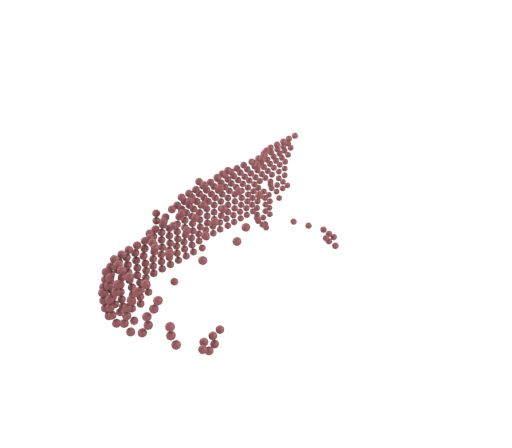
\includegraphics[width=2cm,trim={\cropleft cm \croplower cm \cropright cm \cropupper cm},clip]{data/shapenet/clean/low/165_points}
                    \end{minipage}
                    \begin{minipage}[t]{0.48\textwidth}
                        \vspace{0px}\centering
                        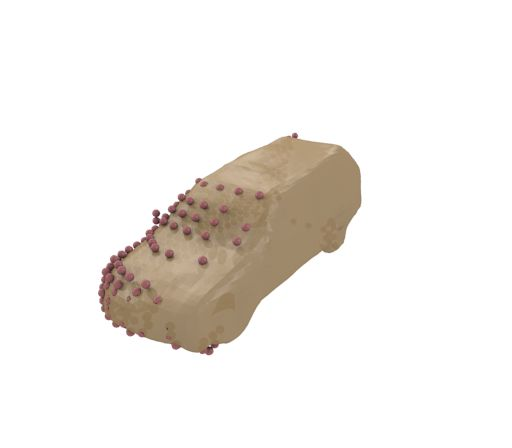
\includegraphics[width=2cm,trim={\cropleft cm \croplower cm \cropright cm \cropupper cm},clip]{experiments/clean.high.10.wide/vae_aml/3_2_results/results_165}
                    \end{minipage}
                \end{minipage}
                \begin{minipage}[t]{0.45\textwidth}
                    \begin{minipage}[t]{0.48\textwidth}
                        \vspace{0px}\centering
                        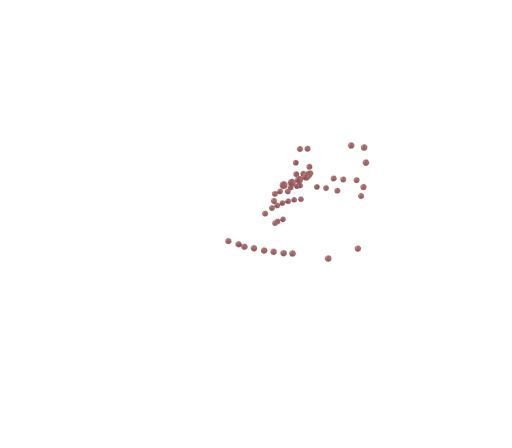
\includegraphics[width=2cm,trim={\cropleft cm \croplower cm \cropright cm \cropupper cm},clip]{data/kitti/1224_points}
                    \end{minipage}
                    \begin{minipage}[t]{0.48\textwidth}
                        \vspace{0px}\centering
                        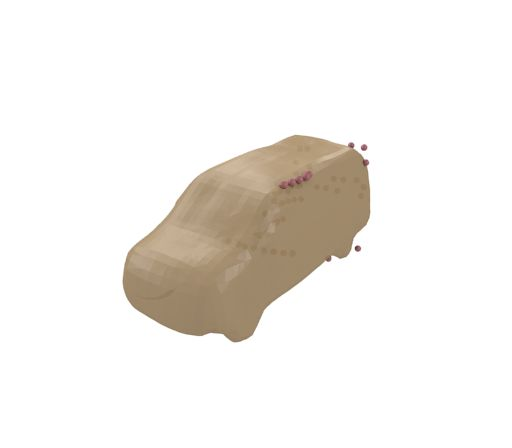
\includegraphics[width=2cm,trim={\cropleft cm \croplower cm \cropright cm \cropupper cm},clip]{experiments/corrected.clean.medium.10.wide.weighted2.1/vae_aml/3_2_results/results_1224}
                    \end{minipage}
                \end{minipage}
                \\[-6px]
                \begin{minipage}[t]{0.45\textwidth}
                    % 264 1188 1452
                    \begin{minipage}[t]{0.48\textwidth}
                        \vspace{0px}\centering
                        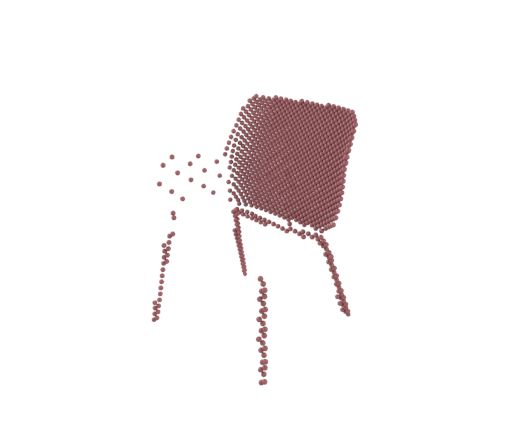
\includegraphics[width=2cm,trim={\cropleft cm \croplower cm \cropright cm \cropupper cm},clip]{data/modelnet/chair/high/1452_points}
                    \end{minipage}
                    \begin{minipage}[t]{0.48\textwidth}
                        \vspace{0px}\centering
                        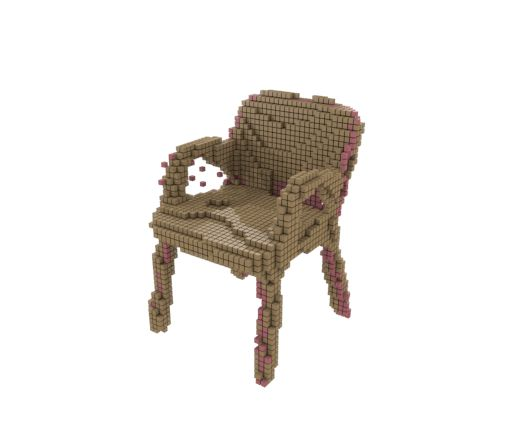
\includegraphics[width=2cm,trim={\cropleft cm \croplower cm \cropright cm \cropupper cm},clip]{experiments/clean.chair.high.10.wide.d/vae_aml/3_3_results/results_1452}
                    \end{minipage}
                \end{minipage}
                \begin{minipage}[t]{0.45\textwidth}
                    \begin{minipage}[t]{0.48\textwidth}
                        \vspace{0px}\centering
                        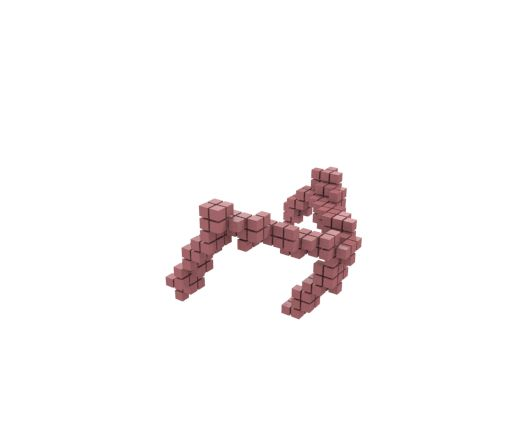
\includegraphics[width=2cm,trim={\cropleft cm \croplower cm \cropright cm \cropupper cm},clip]{data/yang/table/5_bin_points}
                    \end{minipage}
                    \begin{minipage}[t]{0.48\textwidth}
                        \vspace{0px}\centering
                        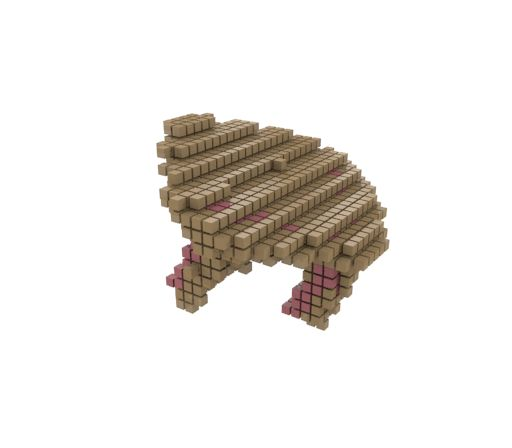
\includegraphics[width=2cm,trim={\cropleft cm \croplower cm \cropright cm \cropupper cm},clip]{experiments/clean.rtable.low.10.wide/vae_aml/3_3_results/results_5}
                    \end{minipage}
                \end{minipage}
            \end{problem}
        \end{minipage}
        \begin{minipage}[t]{0.495\textwidth}
            \strut\vspace*{-\baselineskip} % !
            
            \begin{related}{\large Related Work}
                %{Related work:}
                \begin{itemize}
                    \item Data-driven \cite{Engelmann2016GCPR} -- slow inference;
                    \item Learning-based \cite{Dai2017CVPRa} -- supervision required.
                \end{itemize}
            \end{related}
            \vskip -2mm
            \begin{contribution}{\large Contributions}
                \begin{itemize}
                    \item Learning-based, but weakly-supervised, amortized maximum likelihood ({\bf\color{MPIIorange} AML}) approach.
                    \item Synthetic and real benchmarks.
                    \item[\textcolor{MPIIgreen}{$\blacktriangleright$}] {\color{MPIIgreen} Improved results published in \cite{StutzARXIV2018}.}
                \end{itemize}
            \end{contribution}
        \end{minipage}
        \\[-1mm]
        \begin{minipage}[t]{1\textwidth}
            \strut\vspace*{-\baselineskip}
            
            \begin{method}{\large\bf Method}
                \centering
                \vskip -2mm
                \newcommand{\kittia}{1224}
\newcommand{\kittib}{1530} % 612
\newcommand{\kittic}{0}
\newcommand{\kittid}{2448} % 2754
\newcommand{\kittie}{3366} % 3060

\newcommand{\shapeneta}{0}
\newcommand{\shapenetb}{66}
\newcommand{\shapenetc}{132}
\newcommand{\shapenetd}{198}
\newcommand{\shapenete}{264}
\hspace*{-2mm}
\begin{tikzpicture}
    % ---------------------------------------------------------
    \node[rotate=90] at (7, 0) {\small supervised};
    
    \node[rotate=90] at (-5.2, 0) {\begin{tabular}{c}{\small\bf(1) Shape Prior}\\[1mm]{\footnotesize Variational}\\ {\footnotesize Auto-Encoder \cite{Kingma2014ICLR}}\end{tabular}};
    
    \node[rectangle,draw=black,anchor=west] (prior) at (-4.4,0) {
        \begin{tabular}{c}
	        \includegraphics[height=1cm,trim={\cropleft cm \croplower cm \cropright cm \cropupper cm},clip]{data/shapenet/clean/low/\shapenetb_gt_only}
            \includegraphics[height=1cm,trim={\cropleft cm \croplower cm \cropright cm \cropupper cm},clip]{data/shapenet/clean/low/\shapenetc_gt_only}\\
            \includegraphics[height=1cm,trim={\cropleft cm \croplower cm \cropright cm \cropupper cm},clip]{data/shapenet/clean/low/\shapenetd_gt_only}
            \includegraphics[height=1cm,trim={\cropleft cm \croplower cm \cropright cm \cropupper cm},clip]{data/shapenet/clean/low/\shapenete_gt_only}
        \end{tabular}
    };
    \node[anchor=south] at (-2.85,1.25) {\small Synthetic Training Data};
    
    \node[anchor=south] (y) at (0, 1.25) {\small Shape $y$};
    
    \node[rectangle,draw=black,anchor=west] (input) at (-1, 0) {
        \begin{tabular}{c}
            \includegraphics[height=1cm,trim={\cropleft cm \croplower cm \cropright cm \cropupper cm},clip]{data/shapenet/clean/low/\shapeneta_gt_only}\\
            \includegraphics[height=1cm,trim={\cropleft cm \croplower cm \cropright cm \cropupper cm},clip]{data/shapenet/clean/low/\shapeneta_bin_only}
        \end{tabular}
    };
  
    \draw ($(input.north east) + (0.2,0)$) -- ($(input.north east) + (1.5,-0.75)$) -- ($(input.north east) + (1.5,-1.75)$) -- ($(input.south east) + (0.2,0)$) -- ($(input.north east) + (0.2,0)$);
    \node at ($(input.east) + (0.825,0)$) {\footnotesize encoder};
    
    \node (z) at (2.75, 0) {\small $z$};
    
    \node[rectangle,draw=black,anchor=east] (output) at (6.5, 0) {
        \begin{tabular}{c}
        \includegraphics[height=1cm,trim={\cropleft cm \croplower cm \cropright cm \cropupper cm},clip]{experiments/clean.low.10.wide/prior/3_2_results/results_\shapeneta}\\
        \includegraphics[height=1cm,trim={\cropleft cm \croplower cm \cropright cm \cropupper cm},clip]{experiments/clean.low.10.wide/prior/3_3_results_only/results_\shapeneta}
        \end{tabular}
    };
    
    \draw ($(output.north west) - (0.2,0)$) -- ($(output.north west) - (1.5,0.75)$) -- ($(output.north west) - (1.5,1.75)$) -- ($(output.south west) - (0.2,0)$) -- ($(output.north west) - (0.2,0)$);
    \node at ($(output.west) - (0.825,0)$) {\footnotesize decoder};
    
    \node[anchor=south] (ry) at (5.5, 1.25) {\small Rec. Shape $\tilde{y}$};
    
    \node[] (L) at ($(y) + (2.75,0.4)$) {\small Reconstruction Loss};
    
    \draw[-] (ry) -- ($(ry) + (0,0.4)$);
    \draw[-] ($(ry) + (0,0.4)$) -- (L);
    \draw[-] (y) -- ($(y) + (0,0.4)$);
    \draw[-] ($(y) + (0,0.4)$) -- (L);    
    
    \begin{scope}[shift={(0,-3.5)}]
        % ---------------------------------------------------------
        %\draw[-,MPIIgray] (-6, -2.25) -- (-6, 2) -- (6.75, 2) -- (6.75,-2.25) -- (-6, -2.25);
        \node[rotate=90] at (7, 0) {\small unsupervised};
        
	    \node[rotate=90] at (-5.2, 0) {\begin{tabular}{c}{\small\bf(2) Shape Inference}\\[1mm]{\footnotesize Amortized Maximum}\\{\footnotesize Likelihood ({\bfseries\color{MPIIorange}AML})}\end{tabular}};
	    
	    \node[rectangle,draw=black,anchor=west] (inference) at (-4.4,0) {
	        \begin{tabular}{c}
		        \includegraphics[height=1cm,trim={\cropleft cm \croplower cm \cropright cm \cropupper cm},clip]{data/kitti/\kittib_points}
                \includegraphics[height=1cm,trim={\cropleft cm \croplower cm \cropright cm \cropupper cm},clip]{data/kitti/\kittic_points}
                \\
                \includegraphics[height=1cm,trim={\cropleft cm \croplower cm \cropright cm \cropupper cm},clip]{data/kitti/\kittid_points}
                \includegraphics[height=1cm,trim={\cropleft cm \croplower cm \cropright cm \cropupper cm},clip]{data/kitti/\kittie_points}
	        \end{tabular}
	    };
	    
	    \node[anchor=north] at (-2.85,-1.25) {\small\begin{tabular}{c}Real Training Data\\without Targets\end{tabular}};
	    
	    % --
	    \node(correspondence) at ($(inference) + (0,1.75)$) {\footnotesize\textbf{no correspondence needed}};
	    \draw[-,dotted] (prior) -- (correspondence);
	    \draw[-,dotted] (correspondence) -- (inference);
	    
	    \node(retain) at ($(correspondence) + (6.5,0)$) {\footnotesize retain fixed decoder};
	    \draw[-] ($(prior) + (6.5,-0.9)$) -- (retain);
	    \draw[->] (retain) -- ($(inference) + (6.5,0.9)$);
	    
	    \node[anchor=north] (y) at (0, -1.25) {\small Observation $x$};
	    
	    \node[rectangle,draw=black,anchor=west] (input) at (-1, 0) {
	        \begin{tabular}{c}
	        \includegraphics[height=1cm,trim={\cropleft cm \croplower cm \cropright cm \cropupper cm},clip]{data/kitti/\kittia_points}\\
            \includegraphics[height=1cm,trim={\cropleft cm \croplower cm \cropright cm \cropupper cm},clip]{data/kitti/\kittia_bin_points}
	        \end{tabular}
	    };
	    
	    \draw ($(input.north east) + (0.2,0)$) -- ($(input.north east) + (1.5,-0.75)$) -- ($(input.north east) + (1.5,-1.75)$) -- ($(input.south east) + (0.2,0)$) -- ($(input.north east) + (0.2,0)$);
        \node at ($(input.east) + (0.825,0)$) {\footnotesize \begin{tabular}{c}new\\encoder\end{tabular}};
	    
	    \node (z) at (2.75, 0) {\small $z$};
	    
	    \node[rectangle,draw=black,anchor=east] (output) at (6.5, 0) {
	        \begin{tabular}{c}
	        \includegraphics[height=1cm,trim={\cropleft cm \croplower cm \cropright cm \cropupper cm},clip]{experiments/corrected.clean.medium.10.wide.weighted2.1/vae_aml/3_2_results/results_\kittia}\\
            \includegraphics[height=1cm,trim={\cropleft cm \croplower cm \cropright cm \cropupper cm},clip]{experiments/corrected.clean.medium.10.wide.weighted2.1/vae_aml/3_3_results/results_\kittia}
	        \end{tabular}
	    };
	    
	    \draw ($(output.north west) - (0.2,0)$) -- ($(output.north west) - (1.5,0.75)$) -- ($(output.north west) - (1.5,1.75)$) -- ($(output.south west) - (0.2,0)$) -- ($(output.north west) - (0.2,0)$);
	    \node at ($(output.west) - (0.825,0)$) {\footnotesize \begin{tabular}{c}fixed\\decoder\end{tabular}};
	    
	    \node[anchor=north] (ry) at (5.5, -1.25) {\small Prop. Shape $\tilde{y}$};
	    
	    \node[] (L) at ($(y) - (-2.75,0.4)$) {\small\begin{tabular}{c}Maximum Likelihood Loss\end{tabular}};
	    
	    \draw[-] (ry) -- ($(ry) - (0,0.4)$);
	    \draw[-] ($(ry) - (0,0.4)$) -- (L);
	    \draw[-] (y) -- ($(y) - (0,0.4)$);
	    \draw[-] ($(y) - (0,0.4)$) -- (L);
    \end{scope}
\end{tikzpicture}

            \end{method}
        \end{minipage}
        \\[-4mm]
        \begin{minipage}[t]{1\textwidth}
            \begin{references}{\scriptsize References}
                %{\scriptsize\bf References}
                %\vskip 1mm
                \nocite{Geiger2012CVPR,Chang2015ARXIV,Wu2015CVPR,YangARXIV2018}
                \begingroup
                \RaggedRight
                \setstretch{0.9}
                \renewcommand{\section}[2]{}%
                \color{MPIIdarkergray}
                \printbibliography
                \endgroup
            \end{references}
        \end{minipage}
    \end{minipage}
    \hfill
    \begin{minipage}[t]{0.41\textwidth}
        \strut\vspace*{-\baselineskip} % !
        
        \begin{minipage}[t]{1\textwidth}
            \begin{results}{\large\color{MPIIblue}\bf Results}
                
                \begin{minipage}[t]{0.475\textwidth}
                    \strut\vspace*{-\baselineskip} % !
                    \vspace*{-1.5mm}
                    
                    \begin{tikzpicture}
	\begin{axis}[
    	ybar,
    	% https://tex.stackexchange.com/questions/119887/remove-the-scientific-notation-which-is-unreasonable
    	yticklabel style={
    		/pgf/number format/fixed,
    		/pgf/number format/precision=5
    	},
    	scaled y ticks=false,
    	% https://tex.stackexchange.com/questions/60687/pgfplots-remove-the-plot-line-in-the-legend?utm_medium=organic&utm_source=google_rich_qa&utm_campaign=google_rich_qa
        legend plot pos=none,
    	legend style={
    		at={(-0.1,1)},
    		anchor=south west,
            draw=none,
            font=\footnotesize,
    	},
    	% https://tex.stackexchange.com/questions/48620/pgfplots-alignment-and-size-of-math-in-legend
    	legend cell align=left,
    	xtick={
    		1,
    		2,
            3,
    		4,
            5
    	},
    	xticklabels={
            VAE\\Prior,
    		\cite{Dai2017CVPRa},
    		{\bf\color{MPIIorange} AML},
    		ML,
    		\cite{Engelmann2016GCPR},
    	},
    	x tick label style={text width=1.5cm,align=right,font=\small},
    	ymin=0,
        ymax=4,
    	width=7.2cm,
    	height=3.5cm,
    	enlarge x limits=0.125,
    	% https://tex.stackexchange.com/questions/271027/pgfplots-how-to-rotate-extra-x-tick-labels
    	x tick label style={
    		rotate=90,
    		anchor=east,
    	},
    	bar width=22,
    	% https://tex.stackexchange.com/questions/46316/how-to-put-the-values-of-each-bar-in-a-pgfplots-bar-chart-inside-the-bar-itself
    	nodes near coords,
    	axis lines*=left,
    	y axis line style={opacity=0},
    	yticklabels={\empty},
    	ytick style={draw=none},
    	% https://tex.stackexchange.com/questions/51095/reduce-font-size-and-keep-label-position-in-bar-chart-using-pgf-tikz
    	every node near coord/.append style={
    		font=\footnotesize,
    		% https://tex.stackexchange.com/questions/239132/pgfplots-bar-plot-number-format
    		/pgf/number format/.cd, fixed, precision=3,1000 sep={}
    	},
	]
	
    	% AbsThr
    	\addplot[MPIIblue,fill=MPIIblue] coordinates {
            (1, 0.405) % 0.283 0.527
    		(2, 0.512) % 0.391 0.633
    		(3, 0.6655) % 0.57 0.761
    		(4, 0.727) % 0.625 0.829
    		(5, 1.643) % 1.974 1.312
    	};
    	\addlegendentry{\begin{tabular}{l}{\large\color{MPIIblue} ShapeNet}\\[0.5mm]Accuracy and Completeness [vx] $\downarrow$\end{tabular}}
	\end{axis}
    
    \node (middle) at (2.25,0){};
    \node[anchor=south] at ($(middle) + (0,1.2)$){\footnotesize supervision};
    \node[MPIIblue,anchor=north east] at ($(middle) + (-0.05,1.3)$) {\footnotesize $100\%$};
    \draw[MPIIblue,dashed] ($(middle) + (0,1.2)$) -- ($(middle) + (0,-1)$);
    \node[MPIIblue,anchor=north west] at ($(middle) + (0.05,1.3)$) {\footnotesize $\leq3.86\%$};
\end{tikzpicture}
                \end{minipage}
                \begin{minipage}[t]{0.275\textwidth}
                    \strut\vspace*{-\baselineskip} % !
                    \vspace*{-1.5mm}
                    
                    \begin{tikzpicture}
    \begin{axis}[
        ybar,
        % https://tex.stackexchange.com/questions/119887/remove-the-scientific-notation-which-is-unreasonable
        yticklabel style={
            /pgf/number format/fixed,
            /pgf/number format/precision=5
        },
        scaled y ticks=false,
        % https://tex.stackexchange.com/questions/60687/pgfplots-remove-the-plot-line-in-the-legend?utm_medium=organic&utm_source=google_rich_qa&utm_campaign=google_rich_qa
        legend plot pos=none,
        legend style={
            at={(-0.15,1.4)},
            anchor=north west,
            draw=none,
            font=\footnotesize,
        },
        % https://tex.stackexchange.com/questions/48620/pgfplots-alignment-and-size-of-math-in-legend
        legend cell align=left,
        xtick={
            1,
            2,
            3
        },
        xticklabels={
            VAE\\Prior,
            \cite{Dai2017CVPRa},
            {\bf\color{MPIIorange} AML},
        },
        x tick label style={text width=1.5cm,align=right,font=\small},
        ymin=0,
        ymax=0.2,
        width=4.5cm,
        height=3.5cm,
        enlarge x limits=0.2,
        % https://tex.stackexchange.com/questions/271027/pgfplots-how-to-rotate-extra-x-tick-labels
        x tick label style={
            rotate=90,
            anchor=east,
        },
        bar width=22,
        % https://tex.stackexchange.com/questions/46316/how-to-put-the-values-of-each-bar-in-a-pgfplots-bar-chart-inside-the-bar-itself
        nodes near coords,
        axis lines*=left,
        y axis line style={opacity=0},
        yticklabels={\empty},
        ytick style={draw=none},
        % https://tex.stackexchange.com/questions/51095/reduce-font-size-and-keep-label-position-in-bar-chart-using-pgf-tikz
        every node near coord/.append style={
            font=\footnotesize,
            % https://tex.stackexchange.com/questions/239132/pgfplots-bar-plot-number-format
            /pgf/number format/.cd, fixed, precision=3,1000 sep={}
        },
    ]
    
    % AbsThr
    \addplot[MPIIgreen,fill=MPIIgreen] coordinates {
        (1, 0.023)
        (2, 0.03)
        (3, 0.04)
    };
    \addlegendentry{\begin{tabular}{l}{\color{MPIIgreen}\large ModelNet10}\\[0.5mm]Occupancy Error $\downarrow$\end{tabular}}
    \end{axis}
    \node (middle) at (2,0){};
    \node[anchor=south] at ($(middle) + (0,1.2)$){\footnotesize supervision};
    \node[MPIIgreen,anchor=north east] at ($(middle) + (-0.05,1.3)$) {\footnotesize $100\%$};
    \draw[MPIIgreen,dashed] ($(middle) + (0,1.2)$) -- ($(middle) + (0,-1)$);
    \node[MPIIgreen,anchor=north west] at ($(middle) + (0.05,1.3)$) {\footnotesize $\leq9.71\%$};
\end{tikzpicture}
                \end{minipage}
                \begin{minipage}[t]{0.225\textwidth}
                    \strut\vspace*{-\baselineskip} % !
                    \vspace*{-1.5mm}
                    
                    \begin{tikzpicture}
	\begin{axis}[
    	ybar,
    	% https://tex.stackexchange.com/questions/119887/remove-the-scientific-notation-which-is-unreasonable
    	yticklabel style={
    		/pgf/number format/fixed,
    		/pgf/number format/precision=5
    	},
    	scaled y ticks=false,
    	% https://tex.stackexchange.com/questions/60687/pgfplots-remove-the-plot-line-in-the-legend?utm_medium=organic&utm_source=google_rich_qa&utm_campaign=google_rich_qa
        legend plot pos=none,
    	legend style={
    		at={(-0.15,1.4)},
    		anchor=north west,
            draw=none,
            font=\footnotesize,
    	},
    	% https://tex.stackexchange.com/questions/48620/pgfplots-alignment-and-size-of-math-in-legend
    	legend cell align=left,
    	xtick={
    		1,
    		2,
            3
    	},
    	xticklabels={
    		\cite{Dai2017CVPRa},
    		{\bf\color{MPIIorange} AML},
    		\cite{Engelmann2016GCPR},
    	},
    	x tick label style={text width=1.5cm,align=right,font=\small},
    	ymin=0,
        ymax=1,
    	width=4.5cm,
    	height=3.5cm,
    	enlarge x limits=0.2,
    	% https://tex.stackexchange.com/questions/271027/pgfplots-how-to-rotate-extra-x-tick-labels
    	x tick label style={
    		rotate=90,
    		anchor=east,
    	},
    	bar width=22,
    	% https://tex.stackexchange.com/questions/46316/how-to-put-the-values-of-each-bar-in-a-pgfplots-bar-chart-inside-the-bar-itself
    	nodes near coords,
    	axis lines*=left,
    	y axis line style={opacity=0},
    	yticklabels={\empty},
    	ytick style={draw=none},
    	% https://tex.stackexchange.com/questions/51095/reduce-font-size-and-keep-label-position-in-bar-chart-using-pgf-tikz
    	every node near coord/.append style={
    		font=\footnotesize,
    		% https://tex.stackexchange.com/questions/239132/pgfplots-bar-plot-number-format
    		/pgf/number format/.cd, fixed, precision=3,1000 sep={}
    	},
	]
	
    	% AbsThr
    	\addplot[MPIIred,fill=MPIIred] coordinates {
    		(1, 0.128)
    		(2, 0.12)
    		(3, 0.13)
    	};
    	\addlegendentry{\begin{tabular}{l}{\large\color{MPIIred} KITTI}\\[0.5mm]Completeness [m] $\downarrow$\end{tabular}}
	\end{axis}
    \node (middle) at (0.95,0){};
    \node[anchor=south] at ($(middle) + (0,1.2)$){\footnotesize supervision};
    \node[MPIIred,anchor=north east] at ($(middle) + (-0.05,1.3)$) {\footnotesize $100\%$};
    \draw[MPIIred,dashed] ($(middle) + (0,1.2)$) -- ($(middle) + (0,-1)$);
    \node[MPIIred,anchor=north west] at ($(middle) + (0.05,1.3)$) {\footnotesize $\leq6.79\%$};
\end{tikzpicture}
                \end{minipage}
                \vspace*{-10mm}
            \end{results}
            \vspace*{-1mm}
            \begin{moreresults}{Runtime}
                $\sim2ms$ ({\bf\color{MPIIorange} AML} and \cite{Dai2017CVPRa}, GPU) vs. $>168ms$ (\cite{Engelmann2016GCPR}, CPU with Multi-Threading) and $>30s$ (ML, GPU).
            \end{moreresults}
            \vspace*{-1mm}
            \begin{moreresults}{{ShapeNet and ModelNet (Synthetic, Single Categories)}}
                {\footnotesize
\newcommand{\cleana}{231} % 165 alternative
\newcommand{\cleanb}{297}

\newcommand{\noisya}{132}
\newcommand{\noisyb}{66}

\newcommand{\bathtuba}{792}
\newcommand{\bathtubb}{330}

\newcommand{\chaira}{528}
\newcommand{\chairb}{990} % 0 924

\newcommand{\deska}{264} % 198
\newcommand{\deskb}{858}

\newcommand{\tablea}{858}
\newcommand{\tableb}{396} % 600 594

\hspace*{-6px}
\begin{minipage}[t]{0.02\textwidth}
    \vspace{0px}\centering
    \vspace{4.5mm}
    \rotatebox[]{90}{ShapeNet}
\end{minipage}
\begin{minipage}[t]{0.10\textwidth}
   	\vspace{0px}\centering
   	\hspace*{3mm}
    Obs\\[-1px]
   	\includegraphics[width=1.7cm,trim={\cropleft cm \croplower cm \cropright cm \cropupper cm},clip]{data/shapenet/noisy/low/\noisya_points}
\end{minipage}
\begin{minipage}[t]{0.10\textwidth}
   	\vspace{0px}\centering
   	\hspace*{3mm}
    \cite{Dai2017CVPRa}\\[-1px]
   	\includegraphics[width=1.7cm,trim={\cropleft cm \croplower cm \cropright cm \cropupper cm},clip]{experiments/noisy.low.10.wide.weighted2.1/sup/3_2_results/results_\noisya}
\end{minipage}
\begin{minipage}[t]{0.10\textwidth}
    \vspace{0px}\centering
    \hspace*{3mm}
    \cite{Dai2017CVPRa}\\[-1px]
    \includegraphics[width=1.7cm,trim={\cropleft cm \croplower cm \cropright cm \cropupper cm},clip]{experiments/noisy.low.10.wide.weighted2.1/sup/3_3_results/results_\noisya}
\end{minipage}
\begin{minipage}[t]{0.10\textwidth}
   	\vspace{0px}\centering
   	\hspace*{3mm}
    \scriptsize \cite{Engelmann2016GCPR}/ICP\\[-1px]
   	\includegraphics[width=1.7cm,trim={\cropleft cm \croplower cm \cropright cm \cropupper cm},clip]{experiments/noisy.low.10.wide.weighted2.1/rw/results_\noisya}
\end{minipage}
\begin{minipage}[t]{0.10\textwidth}
    \vspace{0px}\centering
    \hspace*{3mm}
    ML\\[-1px]
    \includegraphics[width=1.7cm,trim={\cropleft cm \croplower cm \cropright cm \cropupper cm},clip]{experiments/noisy.low.10.wide.weighted2.1/ml/3_2_results/results_\noisya}
\end{minipage}
%\begin{minipage}[t]{0.10\textwidth}
%    \vspace{0px}\centering
%    %\ML\\
%    \includegraphics[width=1.7cm,trim={\cropleft cm \croplower cm \cropright cm \cropupper cm},clip]{experiments/noisy.low.10.wide.weighted2.1/ml/3_3_results/results_\noisya}
%\end{minipage}
\begin{minipage}[t]{0.10\textwidth}
   	\vspace{0px}\centering
    \hspace*{3mm}
   	{\bf\color{MPIIorange} AML}\\[-1px]
   	\includegraphics[width=1.7cm,trim={\cropleft cm \croplower cm \cropright cm \cropupper cm},clip]{experiments/noisy.low.10.wide.weighted2.1/vae_aml/3_2_results/results_\noisya}
\end{minipage}
\begin{minipage}[t]{0.10\textwidth}
   	\vspace{0px}\centering
    \hspace*{3mm}
   	{\bf\color{MPIIorange} AML}\\[-1px]
   	\includegraphics[width=1.7cm,trim={\cropleft cm \croplower cm \cropright cm \cropupper cm},clip]{experiments/noisy.low.10.wide.weighted2.1/vae_aml/3_3_results/results_\noisya}
\end{minipage}
\begin{minipage}[t]{0.10\textwidth}
   	\vspace{0px}\centering
    \hspace*{3mm}
   	GT\\[-1px]
   	\includegraphics[width=1.7cm,trim={\cropleft cm \croplower cm \cropright cm \cropupper cm},clip]{data/shapenet/noisy/low/\noisya_gt}
\end{minipage}
\begin{minipage}[t]{0.10\textwidth}
    \vspace{0px}\centering
    \hspace*{3mm}
    GT\\[-1px]
    \includegraphics[width=1.7cm,trim={\cropleft cm \croplower cm \cropright cm \cropupper cm},clip]{data/shapenet/noisy/low/\noisya_bin}
\end{minipage}
\\[-2px]
\hspace*{-6px}
\begin{minipage}[t]{0.02\textwidth}
    \vspace{0px}\centering
    \vspace{4.5mm}
    \rotatebox[]{90}{ShapeNet}
\end{minipage}
\begin{minipage}[t]{0.10\textwidth}
   	\vspace{0px}\centering
   	%Obs\\
   	\includegraphics[width=1.7cm,trim={\cropleft cm \croplower cm \cropright cm \cropupper cm},clip]{data/shapenet/noisy/low/\noisyb_points}
\end{minipage}
\begin{minipage}[t]{0.10\textwidth}
   	\vspace{0px}\centering
   	%\Dai\\
   	\includegraphics[width=1.7cm,trim={\cropleft cm \croplower cm \cropright cm \cropupper cm},clip]{experiments/noisy.low.10.wide.weighted2.1/sup/3_2_results/results_\noisyb}
\end{minipage}
\begin{minipage}[t]{0.10\textwidth}
   	\vspace{0px}\centering
   	%\Dai\\
   	\includegraphics[width=1.7cm,trim={\cropleft cm \croplower cm \cropright cm \cropupper cm},clip]{experiments/noisy.low.10.wide.weighted2.1/sup/3_3_results/results_\noisyb}
\end{minipage}
\begin{minipage}[t]{0.10\textwidth}
   	\vspace{0px}\centering
   	%\Engelmann\\
   	\includegraphics[width=1.7cm,trim={\cropleft cm \croplower cm \cropright cm \cropupper cm},clip]{experiments/noisy.low.10.wide.weighted2.1/rw/results_\noisyb}
\end{minipage}
\begin{minipage}[t]{0.10\textwidth}
    \vspace{0px}\centering
    %\ML\\
    \includegraphics[width=1.7cm,trim={\cropleft cm \croplower cm \cropright cm \cropupper cm},clip]{experiments/noisy.low.10.wide.weighted2.1/ml/3_2_results/results_\noisyb}
\end{minipage}
%\begin{minipage}[t]{0.10\textwidth}
%   	\vspace{0px}\centering
%   	%\ML\\
%   	\includegraphics[width=1.7cm,trim={\cropleft cm \croplower cm \cropright cm \cropupper cm},clip]{experiments/noisy.low.10.wide.weighted2.1/ml/3_3_results/results_\noisyb}
%\end{minipage}
\begin{minipage}[t]{0.10\textwidth}
   	\vspace{0px}\centering
   	%\AML\\
   	\includegraphics[width=1.7cm,trim={\cropleft cm \croplower cm \cropright cm \cropupper cm},clip]{experiments/noisy.low.10.wide.weighted2.1/vae_aml/3_2_results/results_\noisyb}
\end{minipage}
\begin{minipage}[t]{0.10\textwidth}
   	\vspace{0px}\centering
   	%\AML\\
   	\includegraphics[width=1.7cm,trim={\cropleft cm \croplower cm \cropright cm \cropupper cm},clip]{experiments/noisy.low.10.wide.weighted2.1/vae_aml/3_3_results/results_\noisyb}
\end{minipage}
\begin{minipage}[t]{0.10\textwidth}
   	\vspace{0px}\centering
   	%GT\\
   	\includegraphics[width=1.7cm,trim={\cropleft cm \croplower cm \cropright cm \cropupper cm},clip]{data/shapenet/noisy/low/\noisyb_gt}
\end{minipage}
\begin{minipage}[t]{0.10\textwidth}
   	\vspace{0px}\centering
   	%GT\\
   	\includegraphics[width=1.7cm,trim={\cropleft cm \croplower cm \cropright cm \cropupper cm},clip]{data/shapenet/noisy/low/\noisyb_bin}
\end{minipage}
\\[2mm]
\hspace*{-6px}
\begin{minipage}[t]{0.02\textwidth}
    \vspace{0px}\centering
    \vspace{1.5mm}
    \rotatebox[]{90}{ModelNet}
\end{minipage}
\begin{minipage}[t]{0.10\textwidth}
	\vspace{0px}\centering
	%Obs\\
	\includegraphics[width=1.7cm,trim={\cropleft cm \croplower cm \cropright cm \cropupper cm},clip]{data/modelnet/chair/low/\chaira_points}
\end{minipage}
\begin{minipage}[t]{0.10\textwidth}
	\vspace{0px}\centering
	%\Dai\\
	\includegraphics[width=1.7cm,trim={\cropleft cm \croplower cm \cropright cm \cropupper cm},clip]{experiments/clean.chair.low.10.wide/sup/3_2_results/results_\chaira}
\end{minipage}
\begin{minipage}[t]{0.10\textwidth}
	\vspace{0px}\centering
	%\Dai\\
	\includegraphics[width=1.7cm,trim={\cropleft cm \croplower cm \cropright cm \cropupper cm},clip]{experiments/clean.chair.low.10.wide/sup/3_3_results/results_\chaira}
\end{minipage}
\begin{minipage}[t]{0.10\textwidth}
	\vspace{0px}\centering
	%\ICP\\
	\includegraphics[width=1.7cm,trim={\cropleft cm \croplower cm \cropright cm \cropupper cm},clip]{experiments/clean.chair.low.10.wide/icp/3_2_results/results_\chaira}
\end{minipage}
\begin{minipage}[t]{0.10\textwidth}
    \vspace{0px}\centering
    %\ML\\
    \includegraphics[width=1.7cm,trim={\cropleft cm \croplower cm \cropright cm \cropupper cm},clip]{experiments/clean.chair.low.10.wide/ml/3_2_results/results_\chaira}
\end{minipage}
%\begin{minipage}[t]{0.10\textwidth}
%	\vspace{0px}\centering
%	%\ML\\
%	\includegraphics[width=1.7cm,trim={\cropleft cm \croplower cm \cropright cm \cropupper cm},clip]{experiments/clean.chair.low.10.wide/ml/3_3_results/results_\chaira}
%\end{minipage}
\begin{minipage}[t]{0.10\textwidth}
	\vspace{0px}\centering
	%\AML\\
	\includegraphics[width=1.7cm,trim={\cropleft cm \croplower cm \cropright cm \cropupper cm},clip]{experiments/clean.chair.low.10.wide/vae_aml/3_2_results/results_\chaira}
\end{minipage}
\begin{minipage}[t]{0.10\textwidth}
	\vspace{0px}\centering
	%\AML\\
	\includegraphics[width=1.7cm,trim={\cropleft cm \croplower cm \cropright cm \cropupper cm},clip]{experiments/clean.chair.low.10.wide/vae_aml/3_3_results/results_\chaira}
\end{minipage}
\begin{minipage}[t]{0.10\textwidth}
	\vspace{0px}\centering
	%GT\\
	\includegraphics[width=1.7cm,trim={\cropleft cm \croplower cm \cropright cm \cropupper cm},clip]{data/modelnet/chair/low/\chaira_gt}
\end{minipage}
\begin{minipage}[t]{0.10\textwidth}
	\vspace{0px}\centering
	%GT\\
	\includegraphics[width=1.7cm,trim={\cropleft cm \croplower cm \cropright cm \cropupper cm},clip]{data/modelnet/chair/low/\chaira_bin}
\end{minipage}
\\[-2px]
\hspace*{-6px}
\begin{minipage}[t]{0.02\textwidth}
    \vspace{0px}\centering
    \vspace{2.5mm}
    \rotatebox[]{90}{ModelNet}
\end{minipage}
\begin{minipage}[t]{0.10\textwidth}
	\vspace{0px}\centering
	%Obs\\
	\includegraphics[width=1.7cm,trim={\cropleft cm \croplower cm \cropright cm \cropupper cm},clip]{data/modelnet/desk/low/\deska_points}
\end{minipage}
\begin{minipage}[t]{0.10\textwidth}
	\vspace{0px}\centering
	%\Dai\\
	\includegraphics[width=1.7cm,trim={\cropleft cm \croplower cm \cropright cm \cropupper cm},clip]{experiments/clean.desk.low.10.wide/sup/3_2_results/results_\deska}
\end{minipage}
\begin{minipage}[t]{0.10\textwidth}
	\vspace{0px}\centering
	%\Dai\\
	\includegraphics[width=1.7cm,trim={\cropleft cm \croplower cm \cropright cm \cropupper cm},clip]{experiments/clean.desk.low.10.wide/sup/3_3_results/results_\deska}
\end{minipage}
\begin{minipage}[t]{0.10\textwidth}
	\vspace{0px}\centering
	%\ICP\\
	\includegraphics[width=1.7cm,trim={\cropleft cm \croplower cm \cropright cm \cropupper cm},clip]{experiments/clean.desk.low.10.wide/icp/3_2_results/results_\deska}
\end{minipage}
\begin{minipage}[t]{0.10\textwidth}
    \vspace{0px}\centering
    %\ML\\
    \includegraphics[width=1.7cm,trim={\cropleft cm \croplower cm \cropright cm \cropupper cm},clip]{experiments/clean.desk.low.10.wide/ml/3_2_results/results_\deska}
\end{minipage}
%\begin{minipage}[t]{0.10\textwidth}
%	\vspace{0px}\centering
%	%\ML\\
%	\includegraphics[width=1.7cm,trim={\cropleft cm \croplower cm \cropright cm \cropupper cm},clip]{experiments/clean.desk.low.10.wide/ml/3_3_results/results_\deska}
%\end{minipage}
\begin{minipage}[t]{0.10\textwidth}
	\vspace{0px}\centering
	%\AML\\
	\includegraphics[width=1.7cm,trim={\cropleft cm \croplower cm \cropright cm \cropupper cm},clip]{experiments/clean.desk.low.10.wide/vae_aml/3_2_results/results_\deska}
\end{minipage}
\begin{minipage}[t]{0.10\textwidth}
	\vspace{0px}\centering
	%\AML\\
	\includegraphics[width=1.7cm,trim={\cropleft cm \croplower cm \cropright cm \cropupper cm},clip]{experiments/clean.desk.low.10.wide/vae_aml/3_3_results/results_\deska}
\end{minipage}
\begin{minipage}[t]{0.10\textwidth}
	\vspace{0px}\centering
	%GT\\
	\includegraphics[width=1.7cm,trim={\cropleft cm \croplower cm \cropright cm \cropupper cm},clip]{data/modelnet/desk/low/\deska_gt}
\end{minipage}
\begin{minipage}[t]{0.10\textwidth}
	\vspace{0px}\centering
	%GT\\
	\includegraphics[width=1.7cm,trim={\cropleft cm \croplower cm \cropright cm \cropupper cm},clip]{data/modelnet/desk/low/\deska_bin}
\end{minipage}
\\[-2px]
\hspace*{-6px}
\begin{minipage}[t]{0.02\textwidth}
    \vspace{0px}\centering
    \vspace{2.5mm}
    \rotatebox[]{90}{ModelNet}
\end{minipage}
\begin{minipage}[t]{0.10\textwidth}
	\vspace{0px}\centering
	%Obs\\
	\includegraphics[width=1.7cm,trim={\cropleft cm \croplower cm \cropright cm \cropupper cm},clip]{data/modelnet/table/low/\tablea_points}
\end{minipage}
\begin{minipage}[t]{0.10\textwidth}
	\vspace{0px}\centering
	%\Dai\\
	\includegraphics[width=1.7cm,trim={\cropleft cm \croplower cm \cropright cm \cropupper cm},clip]{experiments/clean.table.low.10.wide/sup/3_2_results/results_\tablea}
\end{minipage}
\begin{minipage}[t]{0.10\textwidth}
	\vspace{0px}\centering
	%\Dai\\
	\includegraphics[width=1.7cm,trim={\cropleft cm \croplower cm \cropright cm \cropupper cm},clip]{experiments/clean.table.low.10.wide/sup/3_3_results/results_\tablea}
\end{minipage}
\begin{minipage}[t]{0.10\textwidth}
	\vspace{0px}\centering
	%\ICP\\
	\includegraphics[width=1.7cm,trim={\cropleft cm \croplower cm \cropright cm \cropupper cm},clip]{experiments/clean.table.low.10.wide/icp/3_2_results/results_\tablea}
\end{minipage}
\begin{minipage}[t]{0.10\textwidth}
    \vspace{0px}\centering
    %\ML\\
    \includegraphics[width=1.7cm,trim={\cropleft cm \croplower cm \cropright cm \cropupper cm},clip]{experiments/clean.table.low.10.wide/ml/3_2_results/results_\tablea}
\end{minipage}
%\begin{minipage}[t]{0.10\textwidth}
%	\vspace{0px}\centering
%	%\ML\\
%	\includegraphics[width=1.7cm,trim={\cropleft cm \croplower cm \cropright cm \cropupper cm},clip]{experiments/clean.table.low.10.wide/ml/3_3_results/results_\tablea}
%\end{minipage}
\begin{minipage}[t]{0.10\textwidth}
	\vspace{0px}\centering
	%\AML\\
	\includegraphics[width=1.7cm,trim={\cropleft cm \croplower cm \cropright cm \cropupper cm},clip]{experiments/clean.table.low.10.wide/vae_aml/3_2_results/results_\tablea}
\end{minipage}
\begin{minipage}[t]{0.10\textwidth}
	\vspace{0px}\centering
	%\AML\\
	\includegraphics[width=1.7cm,trim={\cropleft cm \croplower cm \cropright cm \cropupper cm},clip]{experiments/clean.table.low.10.wide/vae_aml/3_3_results/results_\tablea}
\end{minipage}
\begin{minipage}[t]{0.10\textwidth}
	\vspace{0px}\centering
	%GT\\
	\includegraphics[width=1.7cm,trim={\cropleft cm \croplower cm \cropright cm \cropupper cm},clip]{data/modelnet/table/low/\tablea_gt}
\end{minipage}
\begin{minipage}[t]{0.10\textwidth}
	\vspace{0px}\centering
	%GT\\
	\includegraphics[width=1.7cm,trim={\cropleft cm \croplower cm \cropright cm \cropupper cm},clip]{data/modelnet/table/low/\tablea_bin}
\end{minipage}
}
            \end{moreresults}
        \end{minipage}
    \end{minipage}
    \hfill 
    \begin{minipage}[t]{0.21\textwidth}
        \strut\vspace*{-\baselineskip} % !
        
        %\vspace*{-1mm}
        \begin{minipage}{1\textwidth}
            \begin{moreresults}{{ModelNet10 (Synthetic, Multiple Categories)}}
                {\footnotesize
\newcommand{\modelneta}{15318} % 0 7326
\newcommand{\modelnetb}{2664}
\newcommand{\modelnetc}{9324} % 7992
\newcommand{\modelnetd}{18648} % 1998
\newcommand{\modelnete}{9990}
\newcommand{\modelnetf}{5994}
\newcommand{\modelnetg}{12654}
\newcommand{\modelneth}{11988}

\begin{minipage}[t]{0.02\textwidth}
    \vspace{0px}\centering
    \vspace{12mm}
    \rotatebox[]{90}{ModelNet10}
\end{minipage}
\begin{minipage}[t]{0.97\textwidth}
    \vspace{0px}\centering
    \begin{minipage}[t]{0.145\textwidth}
        \vspace{0px}\centering
        \cite{Dai2017CVPRa}\\[-1px]
        \includegraphics[width=1.25cm,trim={\cropleft cm \croplower cm \cropright cm \cropupper cm},clip]{experiments/clean.modelnet10.low.10.wide/sup/3_3_results/results_\modelneta}
    \end{minipage}
    \begin{minipage}[t]{0.145\textwidth}
        \vspace{0px}\centering
        {\bf\color{MPIIorange} AML}\\[-1px]
        \includegraphics[width=1.25cm,trim={\cropleft cm \croplower cm \cropright cm \cropupper cm},clip]{experiments/clean.modelnet10.low.10.wide/vae_aml/3_3_results/results_\modelneta}
    \end{minipage}
    \begin{minipage}[t]{0.145\textwidth}
        \vspace{0px}\centering
        GT\\[-1px]
        \includegraphics[width=1.25cm,trim={\cropleft cm \croplower cm \cropright cm \cropupper cm},clip]{data/modelnet/modelnet10/low/\modelneta_bin}
    \end{minipage}
    \hspace*{2.5mm}
    \begin{minipage}[t]{0.145\textwidth}
        \vspace{0px}\centering
        \cite{Dai2017CVPRa}\\[-1px]
        \includegraphics[width=1.25cm,trim={\cropleft cm \croplower cm \cropright cm \cropupper cm},clip]{experiments/clean.modelnet10.low.10.wide/sup/3_3_results/results_\modelnetb}
    \end{minipage}
    \begin{minipage}[t]{0.145\textwidth}
        \vspace{0px}\centering
        {\bf\color{MPIIorange} AML}\\[-1px]
        \includegraphics[width=1.25cm,trim={\cropleft cm \croplower cm \cropright cm \cropupper cm},clip]{experiments/clean.modelnet10.low.10.wide/vae_aml/3_3_results/results_\modelnetb}
    \end{minipage}
    \begin{minipage}[t]{0.145\textwidth}
        \vspace{0px}\centering
        GT\\[-1px]
        \includegraphics[width=1.25cm,trim={\cropleft cm \croplower cm \cropright cm \cropupper cm},clip]{data/modelnet/modelnet10/low/\modelnetb_bin}
    \end{minipage}
    \\
    \begin{minipage}[t]{0.145\textwidth}
        \vspace{0px}\centering
        \includegraphics[width=1.25cm,trim={\cropleft cm \croplower cm \cropright cm \cropupper cm},clip]{experiments/clean.modelnet10.low.10.wide/sup/3_3_results/results_\modelnetc}
    \end{minipage}
    \begin{minipage}[t]{0.145\textwidth}
        \vspace{0px}\centering
        \includegraphics[width=1.25cm,trim={\cropleft cm \croplower cm \cropright cm \cropupper cm},clip]{experiments/clean.modelnet10.low.10.wide/vae_aml/3_3_results/results_\modelnetc}
    \end{minipage}
    \begin{minipage}[t]{0.145\textwidth}
        \vspace{0px}\centering
        \includegraphics[width=1.25cm,trim={\cropleft cm \croplower cm \cropright cm \cropupper cm},clip]{data/modelnet/modelnet10/low/\modelnetc_bin}
    \end{minipage}
    \hspace*{2.5mm}
    \begin{minipage}[t]{0.145\textwidth}
        \vspace{0px}\centering
        \includegraphics[width=1.25cm,trim={\cropleft cm \croplower cm \cropright cm \cropupper cm},clip]{experiments/clean.modelnet10.low.10.wide/sup/3_3_results/results_\modelnetd}
    \end{minipage}
    \begin{minipage}[t]{0.145\textwidth}
        \vspace{0px}\centering
        \includegraphics[width=1.25cm,trim={\cropleft cm \croplower cm \cropright cm \cropupper cm},clip]{experiments/clean.modelnet10.low.10.wide/vae_aml/3_3_results/results_\modelnetd}
    \end{minipage}
    \begin{minipage}[t]{0.145\textwidth}
        \vspace{0px}\centering
        \includegraphics[width=1.25cm,trim={\cropleft cm \croplower cm \cropright cm \cropupper cm},clip]{data/modelnet/modelnet10/low/\modelnetd_bin}
    \end{minipage}
    \\
    \begin{minipage}[t]{0.145\textwidth}
        \vspace{0px}\centering
        \includegraphics[width=1.25cm,trim={\cropleft cm \croplower cm \cropright cm \cropupper cm},clip]{experiments/clean.modelnet10.low.10.wide/sup/3_3_results/results_\modelnete}
    \end{minipage}
    \begin{minipage}[t]{0.145\textwidth}
        \vspace{0px}\centering
        \includegraphics[width=1.25cm,trim={\cropleft cm \croplower cm \cropright cm \cropupper cm},clip]{experiments/clean.modelnet10.low.10.wide/vae_aml/3_3_results/results_\modelnete}
    \end{minipage}
    \begin{minipage}[t]{0.145\textwidth}
        \vspace{0px}\centering
        \includegraphics[width=1.25cm,trim={\cropleft cm \croplower cm \cropright cm \cropupper cm},clip]{data/modelnet/modelnet10/low/\modelnete_bin}
    \end{minipage}
    \hspace*{2.5mm}
    \begin{minipage}[t]{0.145\textwidth}
        \vspace{0px}\centering
        \includegraphics[width=1.25cm,trim={\cropleft cm \croplower cm \cropright cm \cropupper cm},clip]{experiments/clean.modelnet10.low.10.wide/sup/3_3_results/results_\modelnetf}
    \end{minipage}
    \begin{minipage}[t]{0.145\textwidth}
        \vspace{0px}\centering
        \includegraphics[width=1.25cm,trim={\cropleft cm \croplower cm \cropright cm \cropupper cm},clip]{experiments/clean.modelnet10.low.10.wide/vae_aml/3_3_results/results_\modelnetf}
    \end{minipage}
    \begin{minipage}[t]{0.145\textwidth}
        \vspace{0px}\centering
        \includegraphics[width=1.25cm,trim={\cropleft cm \croplower cm \cropright cm \cropupper cm},clip]{data/modelnet/modelnet10/low/\modelnetf_bin}
    \end{minipage}
\end{minipage}
}
                \vspace*{0.8mm}
            \end{moreresults}
            \vspace*{-1mm}
            \begin{moreresults}{KITTI and Kinect (Real)}
                {\footnotesize
\newcommand{\kittia}{0}
\newcommand{\kittib}{612}
\newcommand{\kittic}{1224}
\newcommand{\kittid}{2754}
\newcommand{\kittie}{3060}
\newcommand{\kittif}{5508} % 5508

\begin{minipage}[t]{0.03\textwidth}
    \vspace{0px}\centering
    \vspace{5mm}
    \rotatebox[]{90}{KITTI}
\end{minipage}
\begin{minipage}[t]{0.145\textwidth}
	\vspace{0px}\centering
    \hspace*{2mm}
	Obs\\[-1px]
	\includegraphics[width=1.45cm,trim={\cropleft cm \croplower cm \cropright cm \cropupper cm},clip]{data/kitti/\kittia_points}
\end{minipage}
\begin{minipage}[t]{0.145\textwidth}
	\vspace{0px}\centering
    \hspace*{2mm}
	\cite{Dai2017CVPRa}\\[-1px]
	\includegraphics[width=1.45cm,trim={\cropleft cm \croplower cm \cropright cm \cropupper cm},clip]{experiments/corrected.clean.medium.10.wide.weighted2.1/sup/3_2_results/results_\kittia}
\end{minipage}
\begin{minipage}[t]{0.145\textwidth}
	\vspace{0px}\centering
    \hspace*{2mm}
	\cite{Engelmann2016GCPR}\\[-1px]
	\includegraphics[width=1.45cm,trim={\cropleft cm \croplower cm \cropright cm \cropupper cm},clip]{experiments/corrected.clean.low.10.wide.weighted2.1/rw/4/results_\kittia}
\end{minipage}
\begin{minipage}[t]{0.145\textwidth}
	\vspace{0px}\centering
    \hspace*{2mm}
	{\bf\color{MPIIorange} AML}\\[-1px]
	\includegraphics[width=1.45cm,trim={\cropleft cm \croplower cm \cropright cm \cropupper cm},clip]{experiments/corrected.clean.medium.10.wide.weighted2.1/vae_aml/3_2_results/results_\kittia}
\end{minipage}
\begin{minipage}[t]{0.145\textwidth}
	\vspace{0px}\centering
    \hspace*{2mm}
	{\bf\color{MPIIorange} AML}\\[-1px]
	\includegraphics[width=1.45cm,trim={\cropleft cm \croplower cm \cropright cm \cropupper cm},clip]{experiments/corrected.clean.medium.10.wide.weighted2.1/vae_aml/3_3_results/results_\kittia}
\end{minipage}
\begin{minipage}[t]{0.145\textwidth}
	\vspace{0px}\centering
    \hspace*{2mm}
	GT\\[-1px]
	\includegraphics[width=1.45cm,trim={\cropleft cm \croplower cm \cropright cm \cropupper cm},clip]{data/kitti/\kittia_gt}
\end{minipage}
\\[-4px]
\begin{minipage}[t]{0.03\textwidth}
    \vspace{0px}\centering
    \vspace{5mm}
    \rotatebox[]{90}{KITTI}
\end{minipage}
\begin{minipage}[t]{0.145\textwidth}
	\vspace{0px}\centering
	%Obs\\
	\includegraphics[width=1.45cm,trim={\cropleft cm \croplower cm \cropright cm \cropupper cm},clip]{data/kitti/\kittib_points}
\end{minipage}
\begin{minipage}[t]{0.145\textwidth}
	\vspace{0px}\centering
	%\Dai\\
	\includegraphics[width=1.45cm,trim={\cropleft cm \croplower cm \cropright cm \cropupper cm},clip]{experiments/corrected.clean.medium.10.wide.weighted2.1/sup/3_2_results/results_\kittib}
\end{minipage}
\begin{minipage}[t]{0.145\textwidth}
	\vspace{0px}\centering
	%\Engelmann\\
	\includegraphics[width=1.45cm,trim={\cropleft cm \croplower cm \cropright cm \cropupper cm},clip]{experiments/corrected.clean.low.10.wide.weighted2.1/rw/4/results_\kittib}
\end{minipage}
\begin{minipage}[t]{0.145\textwidth}
	\vspace{0px}\centering
	%\AML\\
	\includegraphics[width=1.45cm,trim={\cropleft cm \croplower cm \cropright cm \cropupper cm},clip]{experiments/corrected.clean.medium.10.wide.weighted2.1/vae_aml/3_2_results/results_\kittib}
\end{minipage}
\begin{minipage}[t]{0.145\textwidth}
	\vspace{0px}\centering
	%\AML\\
	\includegraphics[width=1.45cm,trim={\cropleft cm \croplower cm \cropright cm \cropupper cm},clip]{experiments/corrected.clean.medium.10.wide.weighted2.1/vae_aml/3_3_results/results_\kittib}
\end{minipage}
\begin{minipage}[t]{0.145\textwidth}
	\vspace{0px}\centering
	%GT\\
	\includegraphics[width=1.45cm,trim={\cropleft cm \croplower cm \cropright cm \cropupper cm},clip]{data/kitti/\kittib_gt}
\end{minipage}
%\\[-4px]
%\begin{minipage}[t]{0.145\textwidth}
%	\vspace{0px}\centering
%	%Obs\\
%	\includegraphics[width=1.45cm,trim={\cropleft cm \croplower cm \cropright cm \cropupper cm},clip]{data/kitti/\kittic_points}
%\end{minipage}
%\begin{minipage}[t]{0.145\textwidth}
%	\vspace{0px}\centering
%	%\Dai\\
%	\includegraphics[width=1.45cm,trim={\cropleft cm \croplower cm \cropright cm \cropupper cm},clip]{experiments/corrected.clean.medium.10.wide.weighted2.1/sup/3_2_results/results_\kittic}
%\end{minipage}
%\begin{minipage}[t]{0.145\textwidth}
%	\vspace{0px}\centering
%	%\Engelmann\\
%	\includegraphics[width=1.45cm,trim={\cropleft cm \croplower cm \cropright cm \cropupper cm},clip]{experiments/corrected.clean.low.10.wide.weighted2.1/rw/4/results_\kittic}
%\end{minipage}
%\begin{minipage}[t]{0.145\textwidth}
%	\vspace{0px}\centering
%	%\AML\\
%	\includegraphics[width=1.45cm,trim={\cropleft cm \croplower cm \cropright cm \cropupper cm},clip]{experiments/corrected.clean.medium.10.wide.weighted2.1/vae_aml/3_2_results/results_\kittic}
%\end{minipage}
%\begin{minipage}[t]{0.145\textwidth}
%	\vspace{0px}\centering
%	%\AML\\
%	\includegraphics[width=1.45cm,trim={\cropleft cm \croplower cm \cropright cm \cropupper cm},clip]{experiments/corrected.clean.medium.10.wide.weighted2.1/vae_aml/3_3_results/results_\kittic}
%\end{minipage}
%\begin{minipage}[t]{0.145\textwidth}
%	\vspace{0px}\centering
%	%GT\\
%	\includegraphics[width=1.45cm,trim={\cropleft cm \croplower cm \cropright cm \cropupper cm},clip]{data/kitti/\kittic_gt}
%\end{minipage}
%\\[-4px]
%\begin{minipage}[t]{0.145\textwidth}
%	\vspace{0px}\centering
%	%Obs\\
%	\includegraphics[width=1.45cm,trim={\cropleft cm \croplower cm \cropright cm \cropupper cm},clip]{data/kitti/\kittid_points}
%\end{minipage}
%\begin{minipage}[t]{0.145\textwidth}
%	\vspace{0px}\centering
%	%\Dai\\
%	\includegraphics[width=1.45cm,trim={\cropleft cm \croplower cm \cropright cm \cropupper cm},clip]{experiments/corrected.clean.medium.10.wide.weighted2.1/sup/3_2_results/results_\kittid}
%\end{minipage}
%\begin{minipage}[t]{0.145\textwidth}
%	\vspace{0px}\centering
%	%\Engelmann\\
%	\includegraphics[width=1.45cm,trim={\cropleft cm \croplower cm \cropright cm \cropupper cm},clip]{experiments/corrected.clean.low.10.wide.weighted2.1/rw/4/results_\kittid}
%\end{minipage}
%\begin{minipage}[t]{0.145\textwidth}
%	\vspace{0px}\centering
%	%\AML\\
%	\includegraphics[width=1.45cm,trim={\cropleft cm \croplower cm \cropright cm \cropupper cm},clip]{experiments/corrected.clean.medium.10.wide.weighted2.1/vae_aml/3_2_results/results_\kittid}
%\end{minipage}
%\begin{minipage}[t]{0.145\textwidth}
%	\vspace{0px}\centering
%	%\AML\\
%	\includegraphics[width=1.45cm,trim={\cropleft cm \croplower cm \cropright cm \cropupper cm},clip]{experiments/corrected.clean.medium.10.wide.weighted2.1/vae_aml/3_3_results/results_\kittid}
%\end{minipage}
%\begin{minipage}[t]{0.145\textwidth}
%	\vspace{0px}\centering
%	%GT\\
%	\includegraphics[width=1.45cm,trim={\cropleft cm \croplower cm \cropright cm \cropupper cm},clip]{data/kitti/\kittid_gt}
%\end{minipage}
%\\[-4px]
%\begin{minipage}[t]{0.145\textwidth}
%	\vspace{0px}\centering
%	%Obs\\
%	\includegraphics[width=1.45cm,trim={\cropleft cm \croplower cm \cropright cm \cropupper cm},clip]{data/kitti/\kittif_points}
%\end{minipage}
%\begin{minipage}[t]{0.145\textwidth}
%	\vspace{0px}\centering
%	%\Dai\\
%	\includegraphics[width=1.45cm,trim={\cropleft cm \croplower cm \cropright cm \cropupper cm},clip]{experiments/corrected.clean.medium.10.wide.weighted2.1/sup/3_2_results/results_\kittif}
%\end{minipage}
%\begin{minipage}[t]{0.145\textwidth}
%	\vspace{0px}\centering
%	%\Engelmann\\
%	\includegraphics[width=1.45cm,trim={\cropleft cm \croplower cm \cropright cm \cropupper cm},clip]{experiments/corrected.clean.low.10.wide.weighted2.1/rw/4/results_\kittif}
%\end{minipage}
%\begin{minipage}[t]{0.145\textwidth}
%	\vspace{0px}\centering
%	%\AML\\
%	\includegraphics[width=1.45cm,trim={\cropleft cm \croplower cm \cropright cm \cropupper cm},clip]{experiments/corrected.clean.medium.10.wide.weighted2.1/vae_aml/3_2_results/results_\kittif}
%\end{minipage}
%\begin{minipage}[t]{0.145\textwidth}
%	\vspace{0px}\centering
%	%\AML\\
%	\includegraphics[width=1.45cm,trim={\cropleft cm \croplower cm \cropright cm \cropupper cm},clip]{experiments/corrected.clean.medium.10.wide.weighted2.1/vae_aml/3_3_results/results_\kittif}
%\end{minipage}
%\begin{minipage}[t]{0.145\textwidth}
%	\vspace{0px}\centering
%	%GT\\
%	\includegraphics[width=1.45cm,trim={\cropleft cm \croplower cm \cropright cm \cropupper cm},clip]{data/kitti/\kittif_gt}
%\end{minipage}
}
                \vspace{5mm}
                
                {\footnotesize
\begin{minipage}[t]{0.03\textwidth}
    \vspace{0px}\centering
    \vspace{4mm}
    \rotatebox[]{90}{Kinect}
\end{minipage}
\begin{minipage}[t]{0.145\textwidth}
    \vspace{0px}\centering
    \hspace*{2mm}
    Obs\\[-1px]
    \includegraphics[width=1.45cm,trim={\cropleft cm \croplower cm \cropright cm \cropupper cm},clip]{data/yang/table/5_bin_points}
\end{minipage}
\begin{minipage}[t]{0.145\textwidth}
    \vspace{0px}\centering
    \hspace*{2mm}
    {\bf\color{MPIIorange} AML}\\[-1px]
    \includegraphics[width=1.45cm,trim={\cropleft cm \croplower cm \cropright cm \cropupper cm},clip]{experiments/clean.rtable.low.10.wide/vae_aml/3_3_results/results_5}
\end{minipage}
\begin{minipage}[t]{0.145\textwidth}
    \vspace{0px}\centering
    \hspace*{2mm}
    Obs\\[-1px]
    \includegraphics[width=1.45cm,trim={\cropleft cm \croplower cm \cropright cm \cropupper cm},clip]{data/yang/table/6_bin_points}
\end{minipage}
\begin{minipage}[t]{0.145\textwidth}
    \vspace{0px}\centering
    \hspace*{2mm}
    {\bf\color{MPIIorange} AML}\\[-1px]
    \includegraphics[width=1.45cm,trim={\cropleft cm \croplower cm \cropright cm \cropupper cm},clip]{experiments/clean.rtable.low.10.wide/vae_aml/3_3_results/results_6}
\end{minipage}
\begin{minipage}[t]{0.145\textwidth}
    \vspace{0px}\centering
    \hspace*{2mm}
    Obs\\[-1px]
    \includegraphics[width=1.45cm,trim={\cropleft cm \croplower cm \cropright cm \cropupper cm},clip]{data/yang/table/8_bin_points}
\end{minipage}
\begin{minipage}[t]{0.145\textwidth}
	\vspace{0px}\centering
    \hspace*{2mm}
    {\bf\color{MPIIorange} AML}\\[-1px]
	\includegraphics[width=1.45cm,trim={\cropleft cm \croplower cm \cropright cm \cropupper cm},clip]{experiments/clean.rtable.low.10.wide/vae_aml/3_3_results/results_8}
\end{minipage}
}
            \end{moreresults}
        \end{minipage}
        \\
        \begin{minipage}{1\textwidth}            
            \begin{conclusion}{\large\bf Conclusion}
                We proposed a learning-based, but weakly-supervised, amortized maximum likelihood ({\bfseries\color{MPIIorange}AML}) approach to 3D shape completion.
                \vskip 2.5mm
                
                \begin{itemize}
                    \item Outperforms data-driven approach \cite{Engelmann2016GCPR};\\ but $84$ times faster.
                    \item Competitive to learning-based approach \cite{Dai2017CVPRa};\\ but up to $96\%$ less supervision.
                \end{itemize}
            \end{conclusion}
        \end{minipage}
        \\ %[-5mm]
        \begin{minipage}[t]{0.775\textwidth}
            \strut\vspace*{-\baselineskip} % !
            
            \begin{code}{}
                Paper, Code and Data:\\
                \large\bf\url{davidstutz.de/cvpr2018}
            \end{code}
        \end{minipage}
        \hfill
        \begin{minipage}[t]{0.2\textwidth}
            \strut\vspace*{-\baselineskip} % !
            
            \vspace*{0.75mm}
            \includegraphics[width=16mm]{gfx/cvpr2018}
        \end{minipage}
    \end{minipage}
\end{document}
